\begin{enumerate}[label=P\arabic*]
	\item\label{item:triangulares:intro}
		Los n\'umeros triangulares son
		$1$, $3$, $6$, $10$, $15$, \dots;
		los n\'umeros cuadrados son
		$1$, $4$, $9$, $16$, $25$, \dots;
		los n\'umeros pentagonales son
		$1$, $5$, $12$, $22$, $35$, \dots.
		Los siguientes diagramas dan nombre a estos n\'umeros:
		\begin{displaymath}
			
\begin{tikzpicture}
				\filldraw
				(0,0) circle (2pt) ;
				% \node[draw, circle, scale=.3, fill=black] at (0,0) {};
			\end{tikzpicture}
			%
			\qquad
			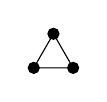
\begin{tikzpicture}
				\filldraw
				(0,0) circle (2pt) --
				(.5,0) circle (2pt) --
				++(120:.5) circle (2pt) -- (0,0) ;
			\end{tikzpicture}
			%
			\qquad
			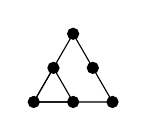
\begin{tikzpicture}
				\filldraw
				(0,0) circle (2pt) --
				(.5,0) circle (2pt) --
				++(120:.5) circle (2pt) --
				(0,0) ;
				\filldraw
				(0,0) --
				(2*.5,0) circle (2pt) --
				++(120:.5) circle (2pt) --
				++(120:.5) circle (2pt) --
				(0,0) ;
			\end{tikzpicture}
			%
			\qquad
			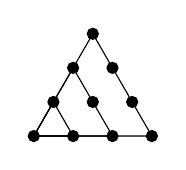
\begin{tikzpicture}
				\filldraw
				(0,0) circle (2pt) --
				(.5,0) circle (2pt) --
				++(120:.5) circle (2pt) --
				(0,0) ;
				\filldraw
				(0,0) --
				(2*.5,0) circle (2pt) --
				++(120:.5) circle (2pt) --
				++(120:.5) circle (2pt) --
				(0,0) ;
				\filldraw
				(0,0) --
				(3*.5,0) circle (2pt) --
				++(120:.5) circle (2pt) --
				++(120:.5) circle (2pt) --
				++(120:.5) circle (2pt) --
				(0,0) ;
			\end{tikzpicture}
			%
		\end{displaymath}
		%
		\begin{displaymath}
			
\begin{tikzpicture}
				\filldraw
				(0,0) circle (2pt) ;
			\end{tikzpicture}
			%
			\qquad
			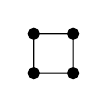
\begin{tikzpicture}
				\filldraw
				(0,0) circle (2pt) ;
				\filldraw
				(0,0) --
				(.5,0) circle (2pt) --
				++(0,.5) circle (2pt) --
				++(-.5,0) circle (2pt) --
				++(0,-.5) ;
			\end{tikzpicture}
			%
			\qquad
			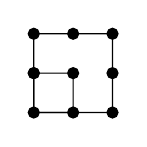
\begin{tikzpicture}
				\filldraw
				(0,0) circle (2pt) ;
				\filldraw
				(0,0) --
				(.5,0) circle (2pt) --
				++(0,.5) circle (2pt) --
				++(-.5,0) circle (2pt) --
				++(0,-.5) ;
				\filldraw
				(0,0) --
				(2*.5,0) circle (2pt) --
				++(0,.5) circle (2pt) --
				++(0,.5) circle (2pt) --
				++(-.5,0) circle (2pt) --
				++(-.5,0) circle (2pt) --
				++(0,-.5) circle (2pt) --
				++(0,-.5) ;
			\end{tikzpicture}
			%
			\qquad
			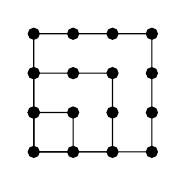
\begin{tikzpicture}
				\filldraw
				(0,0) circle (2pt) ;
				\filldraw
				(0,0) --
				(.5,0) circle (2pt) --
				++(0,.5) circle (2pt) --
				++(-.5,0) circle (2pt) --
				++(0,-.5) ;
				\filldraw
				(0,0) --
				(2*.5,0) circle (2pt) --
				++(0,.5) circle (2pt) --
				++(0,.5) circle (2pt) --
				++(-.5,0) circle (2pt) --
				++(-.5,0) circle (2pt) --
				++(0,-.5) circle (2pt) --
				++(0,-.5) ;
				\filldraw
				(0,0) --
				(3*.5,0) circle (2pt) --
				++(0,.5) circle (2pt) --
				++(0,.5) circle (2pt) --
				++(0,.5) circle (2pt) --
				++(-.5,0) circle (2pt) --
				++(-.5,0) circle (2pt) --
				++(-.5,0) circle (2pt) --
				++(0,-.5) circle (2pt) --
				++(0,-.5) circle (2pt) --
				++(0,-.5) ;
			\end{tikzpicture}
			%
		\end{displaymath}
		%
		\begin{displaymath}
			
\begin{tikzpicture}
				\filldraw
				(0,0) circle (2pt) ;
			\end{tikzpicture}
			%
			\qquad
			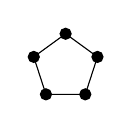
\begin{tikzpicture}
				\filldraw
				(0,0) circle (2pt) ;
				\filldraw
				(0,0) --
				++(.5,0) circle (2pt) --
				++(72:.5) circle (2pt) --
				++(2*72:.5) circle (2pt) --
				++(3*72:.5) circle (2pt) --
				++(4*72:.5) ;
			\end{tikzpicture}
			%
			\qquad
			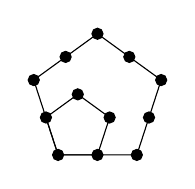
\begin{tikzpicture}
				\filldraw
				(0,0) circle (2pt) ;
				\filldraw
				(0,0) --
				++(.5,0) circle (2pt) --
				++(72:.5) circle (2pt) --
				++(2*72:.5) circle (2pt) --
				++(3*72:.5) circle (2pt) --
				++(4*72:.5) ;
				\filldraw
				(0,0) --
				++(2*.5,0) circle (2pt) --
				++(72:.5) circle (2pt) --
				++(72:.5) circle (2pt) --
				++(2*72:.5) circle (2pt) --
				++(2*72:.5) circle (2pt) --
				++(3*72:.5) circle (2pt) --
				++(3*72:.5) circle (2pt) --
				++(4*72:.5) --
				++(4*72:.5) ;
			\end{tikzpicture}
			%
			\qquad
			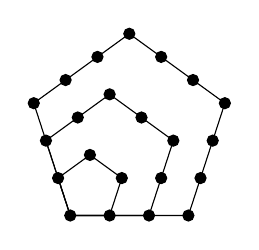
\begin{tikzpicture}
				\filldraw
				(0,0) circle (2pt) ;
				\filldraw
				(0,0) --
				++(.5,0) circle (2pt) --
				++(72:.5) circle (2pt) --
				++(2*72:.5) circle (2pt) --
				++(3*72:.5) circle (2pt) --
				++(4*72:.5) ;
				\filldraw
				(0,0) --
				++(2*.5,0) circle (2pt) --
				++(72:.5) circle (2pt) --
				++(72:.5) circle (2pt) --
				++(2*72:.5) circle (2pt) --
				++(2*72:.5) circle (2pt) --
				++(3*72:.5) circle (2pt) --
				++(3*72:.5) circle (2pt) --
				++(4*72:.5) --
				++(4*72:.5) ;
				\filldraw
				(0,0)  --
				++(3*.5,0) circle (2pt) --
				++(72:.5) circle (2pt) --
				++(72:.5) circle (2pt) --
				++(72:.5) circle (2pt) --
				++(2*72:.5) circle (2pt) --
				++(2*72:.5) circle (2pt) --
				++(2*72:.5) circle (2pt) --
				++(3*72:.5) circle (2pt) --
				++(3*72:.5) circle (2pt) --
				++(3*72:.5) circle (2pt) --
				++(4*72:.5) --
				++(4*72:.5) --
				++(4*72:.5) ;
			\end{tikzpicture}
			%
		\end{displaymath}
		%
		?`Cu\'ales son los primeros n\'umeros hexagonales?
		?`Cu\'ales son los primeros n\'umeros heptagonales?
		?`Cu\'ales son los primeros n\'umeros ``$r$-gonales''?
		Dar f\'ormulas para el $n$-\'esimo n\'umero
		triangular, para el $n$-\'esimo n\'umero cuadrado,
		para el $n$-\'esimo n\'umero pentagonal y, en general,
		para el $n$-\'esimo n\'umero $r$-gonal.
	\item\label{item:triangulares:sumas}
		Probar o refutar las siguientes afirmaciones.
		\begin{enumerate}[label=(\alph*)]
			\item
				Todo entero positivo es, o bien un
				n\'umero triangular, o bien es suma
				de dos o de tres n\'umeros triangulares.
			\item
				Todo entero positivo es suma de, a lo sumo,
				cuatro n\'umeros cuadrados.
			\item
				Todo entero positivo se puede expresar
				como suma de como mucho cinco n\'umeros
				pentagonales.
		\end{enumerate}
		%
		En general, todo entero positivo se puede escribir
		como suma de $r$ o menos n\'umeros $r$-gonales.
	\item\label{item:catalan}
		La ecuaci\'on $2^m-3^n=1$ tiene una cantidad finita
		de soluciones con $m$ y $n$ enteros. M\'as en general,
		si $p$ y $q$ son n\'umeros primos, entonces la
		ecuaci\'on $p^m-q^n=1$ tiene, a lo sumo, una cantidad
		finita de soluciones con $m$ y $n$ enteros
		?`Pod\'es generalizar estas afirmaciones?
	\item\label{item:ciclotomicos}
		Si $p$ es un n\'umero primo, existen polinomios
		irreducibles de cualquier grado, en
		$\polinomios[x]{\Enterosmod[p]}$. Fijado un entero positivo
		$n$, definimos el siguiente polinomio:
		\begin{displaymath}
			P_n(x)\,=\,\prod_f\,f(x)
			\text{ ,}
		\end{displaymath}
		%
		donde el producto se lleva a cabo sobre todos los
		polinomios \emph{m\'onicos} irreducibles de grado
		$n$ en $\polinomios[x]{\Enterosmod[p]}$. Hallar $P_1(x)$.
		Para un $n>0$ general, la siguiente identidad es v\'alida
		en $\polinomios[x]{\Enterosmod[p]}$:
		\begin{displaymath}
			\prod_{d\mid n,d>0}\,P_d(x)\,=\,
				x^{p^n}-x
			\text{ .}
		\end{displaymath}
		%
	\item\label{item:cubica}
		Para cada n\'umero primo $p$ en el rango
		$3<p<20$, calcular el n\'umero $N_p$, que es la
		cantidad de soluciones a la ecuaci\'on
		\begin{math}
			y^2=x^3-x
		\end{math}
		con $x$ e $y$ en $\Enterosmod[p]$. Por ejemplo,
		para $p=5$, $N_5=7$, pues, en $\Enterosmod[5]$,
		las soluciones son
		\begin{displaymath}
			(0,0)\text{ ,}\quad
			(1,0)\text{ ,}\quad
			(2,1)\text{ ,}\quad
			(2,4)\text{ ,}\quad
			(3,2)\text{ ,}\quad
			(3,4)\quad\text{y}\quad
			(4,0)\text{ .}
		\end{displaymath}
		%
		En general, hay una f\'ormula para $N_p$:
		\begin{displaymath}
			N_p\,=\,
				\begin{cases}
					p \text{ ,} &
					\text{si }p\equiv 3\tmodulo[4]
					\text{ ,} \\
					p-2a \text{ ,} &
					\text{si }p\equiv 1\tmodulo[4]
					\text{ y }
					p=a^2+b^2\text{ ,}
				\end{cases}
				%
		\end{displaymath}
		%
		donde $a+b\raizcuarta$ es un primo en
		$\polinomios[\raizcuarta] \Enteros$ congruente
		con $1$ m\'odulo $2+2\raizcuarta$
		?`Pod\'es formular y probar una conjetura en
		relaci\'on con la cantidad de soluciones a la
		ecuaci\'on $y^2=x^3-Dx$ en $\Enterosmod[p]$?
	\item\label{item:cuerpos}
		Investigar qu\'e es un cuerpo finito. Demostrar las
		siguientes afirmaciones.
		\begin{enumerate}[label=(\alph*)]
			\item
				La cantidad de elementos en un \emph{cuerpo finito}
				es una potencia de un n\'umero primo, $p^k$.
			\item
				Para cada primo $p$ y cada entero positivo $k$,
				existe un cuerpo de $p^k$ elementos.
			\item
				Si dos cuerpos finitos tienen la misma cantidad de
				elementos, entonces son \emph{isomorfos}.
			\item
				Todo cuerpo finito tiene una ra\'{\i}z primitiva.
		\end{enumerate}
		%
	\item\label{item:diofanticas}
		Encontr\'a todas las soluciones $(x,y)$, con $x$ e $y$
		enteros a las siguientes ecuaciones:
		\begin{displaymath}
			y^2\,=\,x^3-2 \text{ ;}\quad
			y^2\,=\,x^3+7 \text{ ;}\quad
			y^2\,=\,x^3+1 \text{ .}
		\end{displaymath}
		%
		En cada caso encontrar todas las soluciones con
		$x$ e $y$ \emph{racionales}.
	\item\label{item:cuadraticos}
		Para cada entero $d$ libre de cuadrados, definimos
		el siguiente conjunto
		\begin{math}
			R_d=\big\{a+bw_d\,:\,a,b\in\Enteros\big\}
		\end{math}, donde
		\begin{displaymath}
			w_d\,=\,
				\begin{cases}
					\frac{1+\sqrt d} 2
					\text{ ,} &
					\text{si } d\equiv 1\tmodulo[4]
					\quad\text{y} \\
					\sqrt d \text{ ,} &
					\text{si no.}
				\end{cases}
				%
		\end{displaymath}
		%
		\begin{enumerate}[label=(\alph*)]
			\item
				El conjunto $R_d$ es cerrado por
				multiplicaci\'on y suma, es decir,
				si $x,y\in R_d$, entonces $xy\in R_d$
				y tambi\'en $x+y\in R_d$.
			\item
				Los valores de $d$ para los que $R_d$
				admite un \emph{algoritmo de divisi\'on}
				son una cantidad finita ?`Cu\'ales son?
			\item
				El sistema $R_{-19}$ no posee algoritmo
				de divisi\'on. Sin embargo, es cierto que
				la ecuaci\'on
				\begin{math}
					ax+by=g
				\end{math}
				tiene soluci\'on (en $R_{-19}$), siempre
				que $g$ sea igual al m\'aximo com\'un
				divisor entre $a$ y $b$
				?`Pod\'es demostrarlo?%
				\footnote{
					El Teorema fundamental de la
					Aritm\'etica es consecuencia de la
					resolubilidad de estas ecuaciones.
					As\'{\i}, vemos que dicho Teorema
					es v\'alido en $R_{-19}$, aunque
					no exista en este sistema un
					algoritmo de divisi\'on.
				}
			\item
				Si $p>2$ es un n\'umero primo entero,
				la ecuaci\'on
				\begin{math}
					x^2-xy+
						5y^2=p
				\end{math}
				tiene soluci\'on ($x$ e $y$
				enteras), si y s\'olo si
				$-19$ es un \emph{residuo cuadr\'atico %
				m\'odulo $p$}
				?`Pod\'es generalizar estas ideas?
			\item
				?`Pens\'as que el Teorema fundamental
				es v\'alido en $R_d$ para todo entero
				$d$ libre de cuadrados?
				?`Es cierto que el Teorema fundamental
				es v\'alido en $R_d$ para infinitos $d$?
		\end{enumerate}
		%
		Para una discusi\'on sobre estas preguntas, pod\'es
		consultar, por ejemplo el libro de Hardy y Wright
		\textit{An Introduction to the Theory of Numbers},
		especialmente los cap\'{\i}tulos XIV y XV.
\end{enumerate}
%

